\chapter{Gate-Level Equivalence Checking of Arithmetic Circuits over
Finite Fields}  %$\mathbb{F}_{2^k}$} 
\label{ch:ecbit} 

%Computer algebra techniques have been utilized \cite{lv:date2012} \cite{wienand:cav08} to 
%efficiently solve equivalence verification of arithmetic circuits over Ring ${\mathbb{Z}}_{2^k}$ and 
%Finite field ${\mathbb{F}}_{2^k}$ respectively. These computer algebra based approaches have 
%shown their superority over contemporary BDD/SAT/SMT based methods. 
%The efficiency of \cite{lv:date2012} \cite{wienand:cav08} is achieved by converting 
%an equivalence checking problem to ideal membership testing problem. Combined with 
%circuit topology, the ideal membership testing is further transformed to one single 
%polynomial reduction (polynomial division). Therefore, the stunning results of 
%\cite{lv:date2012} \cite{wienand:cav08} introduce a novel way to solve equivalence 
%verification problem with significant orders of magnitude improvement in runtime. 
%However, \cite{lv:date2012} \cite{wienand:cav08} requires a word level specification 
%to verify against bit-level implementation. This word level information is not always 
%available. In other words, not all specifications can be expressed at word level. 

%To overcome this limitation, we draw inspirations from \cite{lv:date2012} \cite{wienand:cav08}, 
%and derive a general verification approach effective at bit level.

This chapter describes our approach to equivalence checking of two
combinational circuits designed for finite field computations. 
Combinational equivalence checking is 
a fundamental problem in hardware verification, and it has been 
widely investigated over the years. Canonical decision diagrams (BDDs
and their variants), implication-based methods, SAT solvers, and
And-Invert-Graph (AIG) based reductions, are among the many techniques
employed for this purpose. When one circuit is synthesized from the
other, this problem can be efficiently solved using AIG-based
reductions (e.g., the ABC tool \cite{abc}) and circuit-SAT solvers
(e.g., CSAT \cite{csat}). Synthesized circuits generally contain many
sub-circuit equivalences which AIG and CSAT based tools can identify
and exploit for verification. However, when the circuits are
functionally equivalent but structurally very dissimilar, none
of the contemporary techniques,  including ABC and CSAT, offer a
practical solution. Particularly, for {\it custom-designed arithmetic  
  circuits} , this  problem largely remains unsolved today. Since
these custom designed circuits are prevalent in industry, it is
therefore imperative to develop scalable methods to verify such
circuits.   

Focussing on finite field arithmetic circuits, we utilize computer
algebra techniques and formulate the equivalence verification problem
as a  {\it Weak Nullstellensatz proof}, and solve it using Gr\"obner
bases. This requires the computation of a reduced Gr\"obner
basis, which can be expensive for large circuits.  To overcome this
complexity, we again wish to exploit the circuit topology-based term
orderings (as described in the previous chapter) for polynomial
manipulation.  Unfortunately, unlike in the previous case, 
the set of polynomials corresponding to this verification instance
(the miter circuit) does  not constitute a Gr\"obner basis. However,
using Gr\"obner bases theory,  we identify {\it a minimum number of
  S-polynomial computations} that are necessary and sufficient to
prove or disprove equivalence. Experiments demonstrate the
effectiveness and efficiency of our approach --  we can verify
$96$-bit structurally very dissimilar implementations, while none of
the contemporary methods are feasible. 

%%%%%%%%%%%%%%%%%%%%%%%%%%%%%%%%%%%%%%%%%%%%%%%%%%
%%%%%%%%%%%%%%%%%%%%%%%%%%%%%%%%%%%%%%%%%%%%%%%%%%
%%%%%%%%%%%%%%%%%%%%%%%%%%%%%%%%%%%%%%%%%%%%%%%%%%
\section{Problem Statement and Modeling}

In this application, we are given two combinational arithmetic
circuits $C_{1}$ and $C_{2}$, as gate-level flattened netlists. 
We have to prove or disprove their functional equivalence. 

Our approach is generic enough to perform equivalence checking of
any arbitrary combinational arithmetic circuit over
$\mathbb{F}_{2^k}$. However, without loss of generality, we will again
consider finite field multiplier circuits as examples to explain our approach.

Our problem can be formally described as:

\begin{itemize}
\item Given a finite field $\mathbb{F}_{2^k}$, i.e. given $k$ (datapath size), along with the
  corresponding irreducible polynomial $P(x)$. Let $P(\alpha) = 0$,
  i.e. $\alpha$ be the root of $P(x)$.   
\item  Given two $k$-bit combinational circuits $C_{1}$ and $C_{2}$. 
		The common primary inputs of both circuits are $\{a_0,
                \dots, a_{k-1}, ~b_0,\dots, b_{k-1}\}$.  
		The primary outputs of $C_{1}$ are $\{x_0, \dots, x_{k-1}\}$;
		The primary outputs of $C_{2}$ are $\{y_0, \dots, y_{k-1}\}$, 
		where $a_i, b_i, x_i, y_i\in \mathbb{F}_2, i = 0, \dots, k-1$.

\item		The word-level representation of inputs is $A = a_0 +
  a_1 \alpha + \dots + a_{k-1}\alpha^{k-1}$, and $B = b_0 + b_1 \alpha
  + \dots + b_{k-1}\alpha^{k-1}$.  Correspondingly, the outputs are
		$X = x_0 + x_1\alpha  + \dots +  x_{k-1}\alpha^{k-1}$
                and $Y = y_0 + y_1\alpha  + \dots +
                y_{k-1}\alpha^{k-1}$. 
\end{itemize}
Our goal is to formally prove that $\forall a_{i},b_{i} \in
\mathbb{F}_{2} \subset \mathbb{F}_{2^k}$, the outputs $X$ and $Y$ of
circuits $C_{1}$ and $C_{2}$ are equal to each other,  i.e., $ X=Y$
always holds. Otherwise, there must exist a bug in one of the given
circuits.   


\begin{figure}[htb]
\centerline{
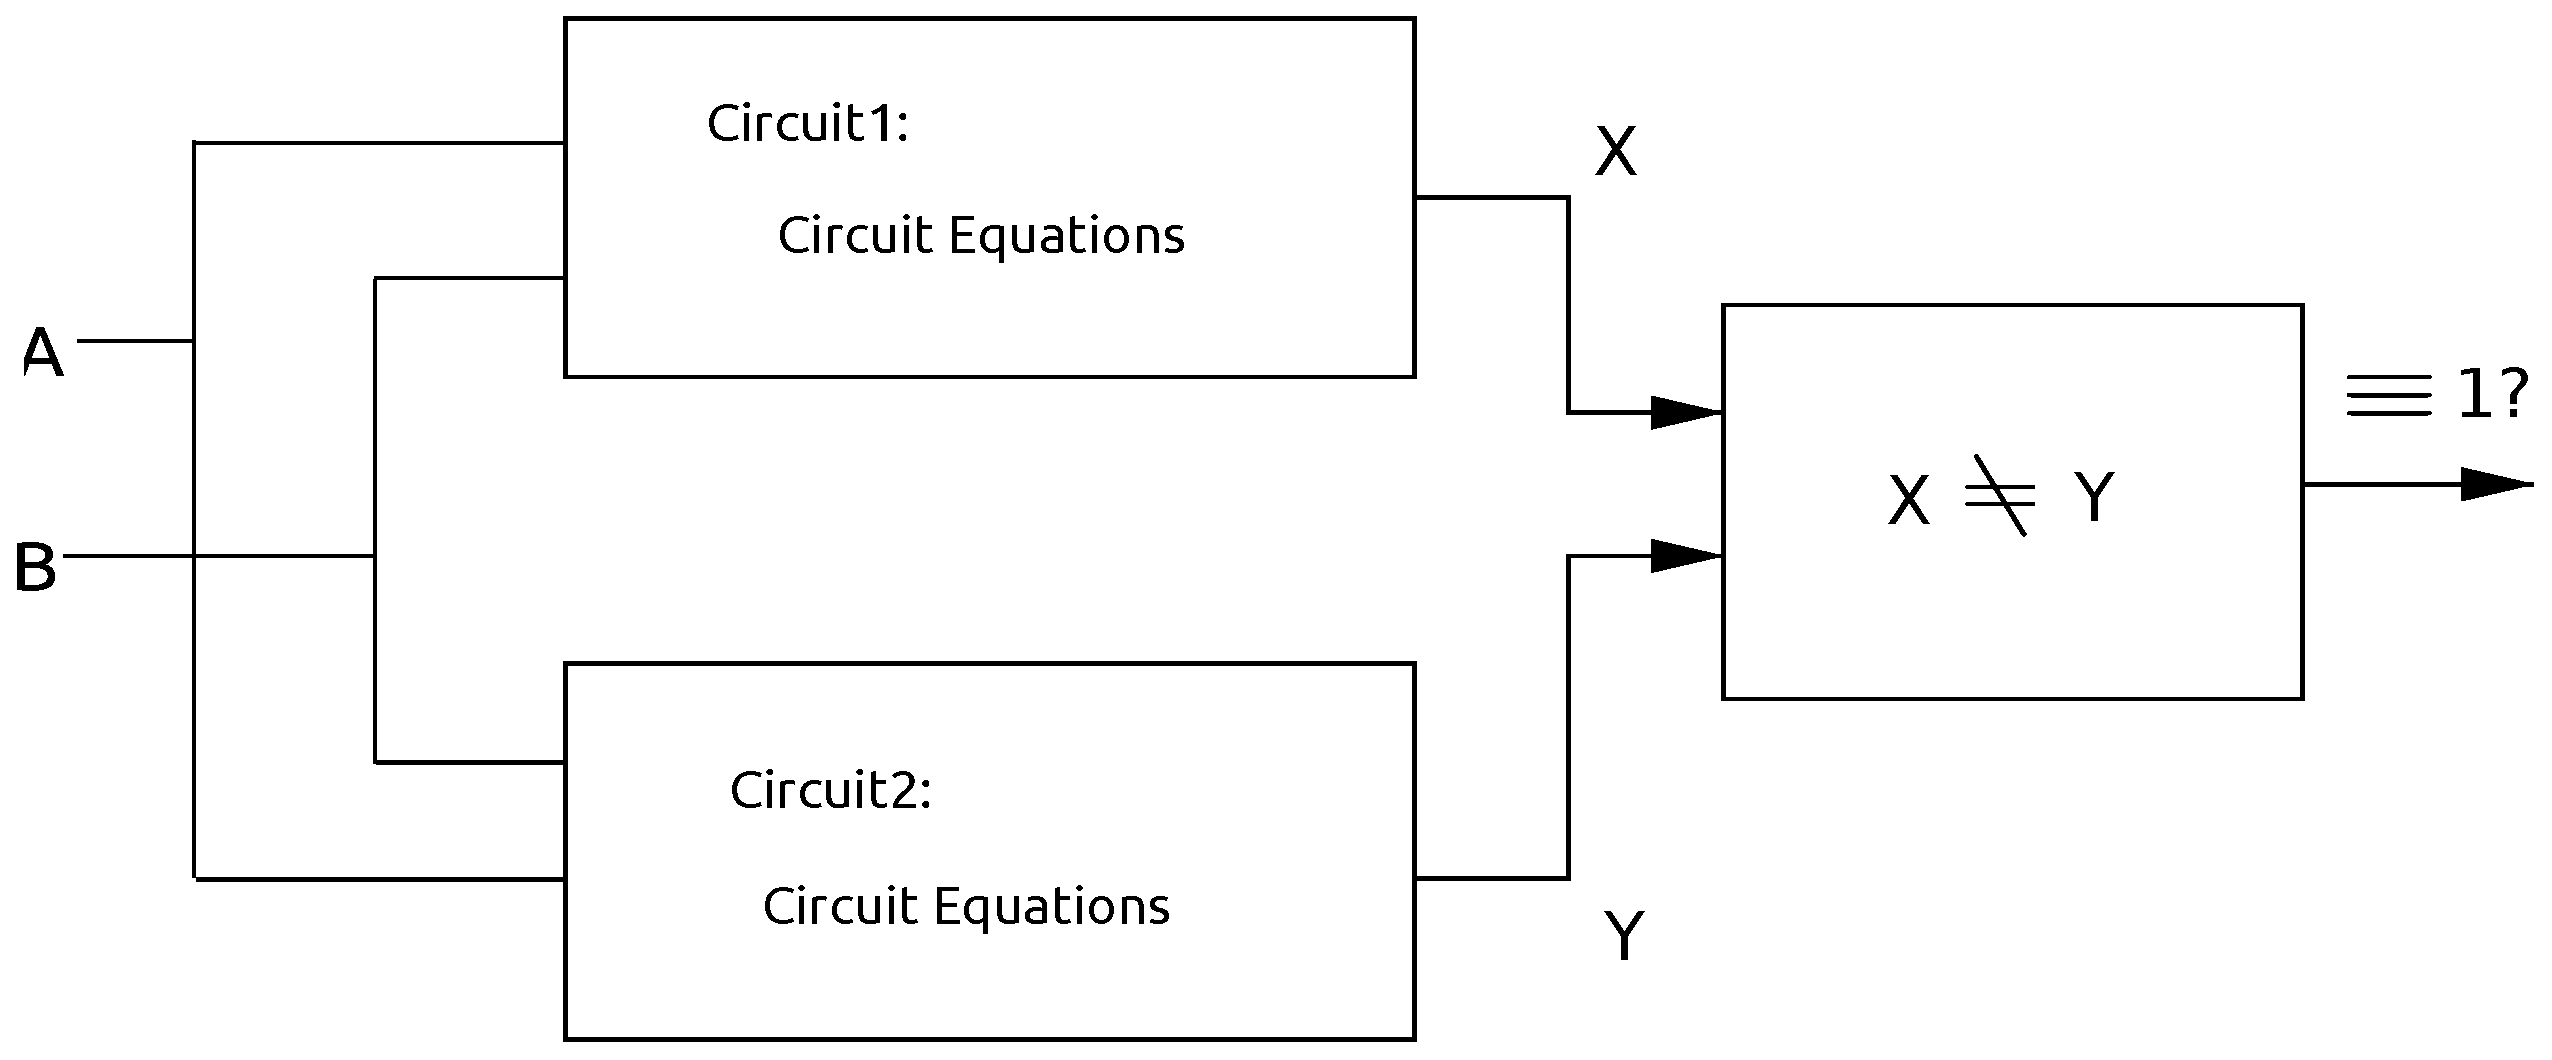
\includegraphics[scale=0.3]{./figures/miter.eps}
}
\caption{The Equivalence Checking Setup: Miter}
\label{fig:miter}
\end{figure}

The equivalence verification setup is shown in Fig. \ref{fig:miter}. 
Given circuits $C_{1}$ and $C_{2}$, 
we want to prove that for all possible inputs, 
the output $X$ of circuit $C_{1}$ is always equal to the output $Y$ of circuit $C_{2}$ . 
This can be, conversely, modeled as proving that $X \neq Y$ has no
solutions. Such a setup is called a ``miter'' circuit, and proving
infeasibility of the miter is a standard practice in combinational
circuit verification. This is mostly because it enables the use of
{\it constraint-solvers} (such as SAT solvers) to prove/disprove
equivalence.  

The constraints for circuits $C_1$ and $C_2$ are modeled as
polynomials over $\mathbb{F}_{2^k}$ using Equations \ref{b2poly}. 
The $X\neq Y$ constraint corresponding to the miter is also modeled as
a polynomial in $\mathbb{F}_{2^k}$ as follows:
\begin{equation}
t(X - Y) = 1, \text{where $t$ is a free variable in }\mathbb{F}_{2^k}  
\end{equation}
The correctness of the above
constraint modeling can be shown as follows: 
\begin{itemize}
	\item When $X = Y, X-Y =0$, so $t\cdot 0 = 1$ has no
          solutions, and the miter is infeasible.
	\item When $X\neq Y, (X-Y) \neq 0$. Over any field, every
          non-zero element has a multiplicative inverse. Let $t^{-1} =
          (X-Y)$. Then $t \cdot t^{-1} = 1$ will always have a
          solution over $\mathbb{F}_{2^k}$. 
\end{itemize} 
% If indeed there are no solutions to $X \neq Y$, then it
% implies that $X$ is always equal to $Y$. Otherwise, 
% if there is a solution to our problem instance, then there is an assignment where
% $X$ differs from $Y$ which indicates a bug in the circuit.   

The above $t(X-Y) = 1$ model for the miter can also be employed over 
$\mathbb{F}_{2}$, i.e. the Boolean ring. Since $1$ is the only
non-zero element in $\mathbb{F}_{2}, t = 1$, and the $X\neq Y$
constraint is specified as $X+Y+1 = 0 \pmod 2$.	  
%\item As a special case over $\mathbb{F}_2$, 

%Following the mapping rules given in Equations \ref{b2poly}, 
%the circuit equations are transformed into polynomial representation.

Overall, the entire miter circuit can be modeled as a polynomial system over
$\mathbb{F}_{2^k}$: 

\begin{eqnarray}\label{eqn:miterbit}
 \left .  \begin{aligned}
f_1^{1}(x_1,x_2,\cdots, x_d)  \\
\vdots  \\
f_A: A + a_0 +  a_1 \alpha + \dots + a_{k-1}\alpha^{k-1}\\
f_{X}: X+x_{0}+x_{1}\cdot \alpha+\dots+ x_{k-1}\cdot \alpha^{k-1} \\
%f_{Z}: Z+z_{0}+z_{1}\cdot \alpha,\cdots,{z_{k-1}}\cdot \alpha^{k-1}=0   
 \end{aligned} 
\ \right\}
 &\qquad&  \text{\it Circuit $1$} \nonumber \\
 \left . \begin{aligned}
f_1^{2}(x_1,x_2,\cdots, x_d)=0  \\
\vdots  \\
f_B: B + b_0 +  b_1 \alpha + \dots + b_{k-1}\alpha^{k-1}\\
f_{Y}: Y+y_{0}+y_{1}\cdot \alpha+\dots+ y_{k-1}\cdot \alpha^{k-1} \\
 \end{aligned} 
\right\}
 &\qquad&  \text{\it  Circuit $2$}  \\
 \left .  \begin{aligned}
f_{m}:t\cdot (X-Y)+1=0  \nonumber 
 \end{aligned} 
\right\}
 &\qquad& \text{Miter:}X \neq Y \nonumber 
\end{eqnarray}

Subsequently, we need to check whether or not there are any solutions
to the set of polynomials in Equations \ref{eqn:miterbit}. The
following example illustrates our polynomial system 
modeling. 

\begin{Example}\label{exp:miter}
Consider two functionally equivalent circuits 
%implementing $2$-bit adder 
over $\mathbb{F}_{2^2}$. The miter is shown in Figure
\ref{fig:2bitadder}. 
	\begin{figure}[htb]
		\centerline{
		\includegraphics[scale=0.35]{./figures/2bitadder.eps}
		}
		\caption{Miter for $2$-bit circuit equivalence.}
		\label{fig:2bitadder}
	\end{figure}

%Then the miter circuit described in Figure \ref{fig:2bitadder} is
The miter is modeled as a system of polynomials, where the outputs of
$C_1, C_2$ are expressed at word level as: $X+x_{0}+x_{1}\cdot \alpha$ and
$Y+y_{0}+y_{1}\cdot \alpha$. 

\begin{eqnarray}%[htb]
 \left .  \begin{aligned}
	x_0&=a_0 \oplus b_0  \Rightarrow x_0+a_0 + b_0 \\
	c_0&=a_0\wedge b_0   \Rightarrow c_0+a_0 \cdot b_0\\
	c_1&=a_0\oplus b_1   \Rightarrow c_1+a_0 + b_1 \\
	x_{1}&=c_{0}\oplus c_{1}  \Rightarrow x_{1}+c_{0}+ c_{1} \\
	&X+x_{0}+x_{1}\cdot \alpha				\\
	 \end{aligned} 
\ \right\}
 &\qquad&  \text{\it Circuit $1$} \nonumber \\
 \left . \begin{aligned}
d_{0}&=\neg (a_{0} \wedge b_{0}) \Rightarrow d_{0}+ a_{0} \cdot b_{0}+1  \\
	d_{1}&=\neg (a_{1} \wedge b_{1}) \Rightarrow d_{1}+ a_{1} \cdot b_{1}+1  \\
	d_{2}&= a_{0} \wedge b_{0} \Rightarrow d_{2}+ a_{0}\cdot b_{0} \\
	d_{3}&=\neg (a_{1} \wedge d_{1}) \Rightarrow d_{3}+ a_{1} \cdot d_{1}+1  \\
	d_{4}&=\neg (b_{1} \wedge d_{1}) \Rightarrow d_{4}+ b_{1} \cdot d_{1}+1  \\
	d_{5}&=\neg (a_{0} \wedge d_{0}) \Rightarrow d_{5}+ a_{0} \cdot d_{0}+1  \\
	d_{6}&=\neg (b_{0} \wedge d_{0}) \Rightarrow d_{6}+ b_{0} \cdot d_{0}+1  \\
	d_{7}&=\neg (d_{3} \wedge d_{4}) \Rightarrow d_{7}+ d_{3} \cdot d_{4}+1  \\ 
	y_{0}&=\neg (d_{5} \wedge d_{6}) \Rightarrow y_{0}+ d_{5} \cdot d_{6}+1  \\
	y_{1}&=d_{2} \oplus d_{7}   \Rightarrow  y_{1}+d_{2} + d_{7}	\\
	&Y+y_{0}+y_{1}\cdot \alpha				\\
 \end{aligned} 
\right\}
 &\qquad&  \text{\it  Circuit $2$} \nonumber \\
 \left .  \begin{aligned}
	&t\cdot (X-Y)+1=0 				
 \end{aligned} 
\right\}
 &\qquad& \text{Miter:}X \neq Y
\end{eqnarray}

\end{Example}


With the polynomial model given above, we formulate our problem as a {\bf Weak Nullstellensatz} problem, 
which is described next.

%%%%%%%%%%%%%%%%%%%%%%%%%%%%%%%%%%%%%%%%%%%%%%%%%%%%%%%%%%%%%%%%
%%%%%%%%%%%%%%%%%%%%%%%%%%%%%%%%%%%%%%%%%%%%%%%%%%%%%%%%%%%%%%%%
%%%%%%%%%%%%%%%%%%%%%%%%%%%%%%%%%%%%%%%%%%%%%%%%%%%%%%%%%%%%%%%%
\subsection{Verification Problem Formulation as Weak Nullstellensatz}

As described in Equation \ref{eqn:miterbit} and Example \ref{exp:miter},
to formulate our verification test, we first analyze the miter circuit and 
model the Boolean gate-level operators as polynomials over $\mathbb{F}_2$
-- i.e. two set of implementation polynomials representing $C_{1}$ and $C_{2}$, 
and the miter polynomials: $X \neq Y$ ($X,Y$ are outputs of $C_{1}$ and $C_{2}$). 
Subsequently, we can reason whether or not solutions exist
to this polynomial system. 

For this purpose, we wish to use techniques from computer algebra and
algebraic geometry to reason about the solutions (variety) to the
polynomial equations (ideal).  

{\bf {Notation:}} Let $F_1, F_2$ represent the set of
polynomials 
generated from circuit $C_1$ and 
$C_2$, respectively. Let $f_m$ represent the miter polynomial. Let
$F=\{F_1,F_2,f_m\}=\{f_1,f_2,\ldots,f_s, f_m\}$ denote this set of
polynomials derived from the miter circuit.  Let $\{x_1,\dots,x_d\}$
denote all variables occurring in $F$. Let $J = \langle
F_1,F_2, f_m\rangle \subset \mathbb{F}_{2^k}[x_{1},\dots,x_{d}]$
denote the ideal generated by these polynomials. 
Subsequently, $V_{\mathbb{F}_{2^k}}(J)$ denotes the variety
(solutions) of $J$ over $\mathbb{F}_{2^k}$. 

Our verification problem
can be formulated as the evaluation: 
\begin{equation}
V_{\mathbb{F}_{2^k}}(J)=\emptyset?
\end{equation}
%To solve this problem, A direct answer is {\bf Weak Nullstellensatz} 


{\it Weak  Nullstellensatz} \cite{null:1890} explicitly specifies the
condition when variety is empty. 

%%%%%%%%%%%%%%%%weak nullstellensatz%%%%%%%%%%%%%
\begin{Theorem}
$\left[\bf{Weak\  Nullstellensatz}\right]$ Let $J \subset \overline
{\mathbb{K}}[x_1, x_2, \cdots, x_d]$ be an ideal satisfying
$V_{\overline{\mathbb{K}}}(J)=\emptyset$. Then $I=\overline {\mathbb{K}}[x_1,
x_2, \cdots, x_n] \iff \{1\} \in J$. 
\end{Theorem}

Recall that a reduced Gr\"obner basis is a canonical representation of
an ideal.  We know that the unit ideal $\langle 1 \rangle$ can 
generate the entire set of polynomials in $\overline{\mathbb{K}}[x_1,
x_2, \cdots, x_n]$.  Therefore, Weak Nullstellensatz can be further
described vis Gr\"obner basis as:

\begin{Corollary}\label{cor:wnf2}
$\left[\bf{Weak\  Nullstellensatz}\right]$ Let $I \subset \overline
{\mathbb{K}}[x_1, x_2, \cdots, x_d]$ be an ideal satisfying
$V(I)=\emptyset$.  Then the Reduced Gr\"obnerBasis(I)$=\{1\}$.
\end{Corollary}

The {\it Weak Nullstellensatz} now offers us a way to evaluate whether
the system of multivariate polynomial equations has a common solution
in ${\overline {\mathbb{K}}}^d$. 

However, {\it Weak Nullstellensatz} is stated over an algebraically
closed field $\overline{\mathbb{K}}$.
Our problem is modeled over $\mathbb{F}_{2^{k}}$ which is not 
algebraically closed. Therefore, {\it Weak Nullstellensatz} will bound
to fail when applied directly, without modification, to finite fields. 

Let us explain why {\it Weak Nullstellensatz} fails when applying to
the field $F_{2}\subset F_{2^{k}}$ by an example. 
\begin{Example} \label{exp:wnfail}
We are given an implementation of a circuit over $\mathbb{F}_2 \subset \mathbb{F}_{2^{k}}$: 
\begin{equation}
x_1=a \vee (\neg a \wedge b)
\end{equation}
Its corresponding specification is :
\begin{equation}
y_1=a \vee b
\end{equation}
where $x_1$ and $y_1$ are symbolically different but functionally equivalent.  
Then we transform the circuit equations into their polynomial forms:
\begin{eqnarray}
x_1=a \vee (\neg a \wedge b) &\mapsto& x_1 + a + b\cdot (a+1) + a\cdot b \cdot (a+1) \pmod 2 \nonumber \\
y_1=a \vee b  &\mapsto& y_{1}+a+b+a\cdot b \pmod 2 \nonumber \\
x_1 \neq y_{1}  &\mapsto& x_1+y_1+1 \pmod 2 \nonumber
\end{eqnarray}
\end{Example}
Then the reduced Gr\"obner basis of above polynomials with term
ordering {\it lex} $x_{1}>y_{1}>a>b$ is:  
\begin{eqnarray}
a^{2}\cdot b+a \cdot b+1 \nonumber \\
y_{1}+a \cdot b+a+b \nonumber \\
x_{1}+a \cdot b+a+b+1 \nonumber 
\end{eqnarray}

which is not equal to $\langle 1\rangle$, even though their variety is
empty. The reason for this can be explained as follows. 

\begin{figure}[htb]
\centerline{
\includegraphics[scale=1]{./figures/closure.eps}
}
\caption{ A Solution (Bug) in
  $(\overline{\mathbb{F}_{2^{k}}}-\mathbb{F}_{2^k})$ is a ``don't
  care''.} 
\label{fig:closure}
\end{figure}

As shown in Figure \ref{fig:closure}, $\overline{ \mathbb{F}_{2^k} }$
is the algebraic closure of $\mathbb{F}_{2^k}$.
If there is no solution to ideal $J$ in the algebraic closure
$\overline{ \mathbb{F}_{2^k}}$,  then there is no solution in
$\mathbb{F}_{2^k}$ either. However, what happens when there is a
solution in $\overline{ \mathbb{F}_{2^k}}$, i.e. $1 \notin GB(J)$?  
In this case, it means that there is a {\it non-empty set of
  solutions} to the polynomial system in
$\overline{\mathbb{F}_{2^k}}^d$. There are two possibilities:  
\begin{itemize}
	\item The solution(s) may lie within $\mathbb{F}_{2^k}^d$.
	\item The solution(s) may lie in $\overline
          {\mathbb{F}_{2^k}}^d$, but outside $\mathbb{F}_{2^k}^d$, as
          depicted in  Fig. \ref{fig:closure}. 
\end{itemize}
We are interested in finding out whether or not $X \neq Y$ over $\mathbb{F}_{2^{k}}$ 
-- i.e. whether the circuit has bugs over the given field
$\mathbb{F}_{2^{k}}$. We do not care if the solution is outside the
field $\mathbb{F}_{2^{k}}$, in which case the bug is really a ``don't
care'' condition (akin to a ``false negative'' in design verification
parlance).  


To address this problem, {\it Weak Nullstellensatz} needs to be suitably
modified for application over finite fields $\mathbb{F}_{2^{k}}$. 
%%%%%%%%%%%%%%%%weak nullstellensatz in finite field%%%%%%%%%%%%%
\begin{Theorem}\label{wnull:ff}
$[\bf{Weak~Nullstellensatz~in~\mathbb{F}_{2^k}}]$\\
Given $f_1,f_2,\cdots,f_s \in \mathbb{F}_{2^k}[x_1,x_2,\cdots,x_d]$. 
Let $J=\langle f_1,f_2,\cdots,f_s\rangle \subset \mathbb{F}_{2^k}[x_1,
x_2, \cdots, x_d]$ be an ideal. Let $J_0 = \langle 
x_1^{2^k}-x_1,x_2^{2^k}-x_2,\cdots,x_d^{2^k}-x_d \rangle$ be the ideal
of vanishing polynomials in $\mathbb{F}_{2^k}$. Then
$V_{\mathbb{F}_{2^k}}(J) = V_{\overline {\mathbb{F}_{2^k}}}(J +
J_0)=\emptyset$,  if and only if the reduced
Gr\"obnerBais$(J+J_{0})=\{1\}$. 
\end{Theorem}
 
\begin{Proof}
%For convenience, let $J_0$ denote $x_1^{2^k}-x_1,x_2^{2^k}-x_2,\cdots,x_d^{2^k}-x_d$.
According to the definition of vanishing polynomials over
$\mathbb{F}_{2^k}$, we have $V_{\overline
  {\mathbb{F}_{2^k}}}(J_0)={\mathbb{F}_{2^k}^d}$. 
From Lemma \ref{lem:closure}, we know:
\begin{equation}
	V_{\overline {\mathbb{F}_{2^k}}}(J+J_0)=V_{\mathbb{F}_{2^k}}(J). 
\end{equation}
Combining with Corollary \ref{cor:wnf2}, we conclude:
\begin{equation}
V_{\overline {\mathbb{F}_{2^k}}}(J+J_0)=\emptyset \Leftrightarrow
\text{ reduced Gr\"obnerBais}(J+J_0) =\langle 1\rangle 
\end{equation}
% Therefore, 
% \begin{equation}
% V_{\overline {\mathbb{F}_{2^k}}}(J+J_0)=V_{\mathbb{F}_{2^k}}(J)=\emptyset \Leftrightarrow {\text{Reduced Gr\"obnerBais(J+$J_{0}$)}}=\{ 1\}  \nonumber
% \end{equation}
%{}
\end{Proof}

\begin{Example}
Re-visiting Example \ref{exp:wnfail}, we need to append the vanishing
polynomials $a^2-a,b^2-b,x_1^2-x_1,y_1^2-y_1$ to given ideal.  Now
when we compute the reduced Gr\"obner basis, we get: reduced-GB$(x_1+
a + b\cdot(a+1) + a\cdot b\cdot(a+1),y_1+a+b+a\cdot
b,x_1+y_1+1,a^2-a,b^2-b,x_1^2-x_1,y_1^2-y_1)=\{1\}$ which proves
$x_1=y_1$. 
\end{Example}


{\bf Verification Problem Formulation:}
Through Weak Nullstellensatz over $\mathbb{F}_{{2^k}}$, given an ideal
$J \in \mathbb{F}_{2^k}[x_{1},\dots,x_{d}]$,  we can determine whether
the variety of $J$ is empty by analyzing the corresponding reduced
Gr\"obner basis of $J+J_0$. 

For our verification problem, we take the polynomials $\{F_1, F_2,
f_m\} = \{f_1, \dots, f_s, f_m\}$  representing the miter circuit
constraints to generate ideal $J$. Then we append the vanishing
polynomials $\{x_1^{2^k} - x_1, \dots, x_d^{2^k} - x_d\}$ of ideal
$J_0$. We compute the reduced Gr\"{o}bner basis $G$ of $J+J_0$ and
check if $G$ equals to the unit ideal $\{1\}$. The two circuits are
functionally equivalent if and only if $G = \{1\}$.

The critical issue in the Weak Nullstellensatz formulation is the
computational complexity of a Gr\"obner basis (as given in
Theorem \ref{thm:gb-complexity}). 
%However, the complexity of Gr\"obner basis makes such a computation
%infeasible.  
To overcome this complexity, we again wish to exploit our
circuit topology-based term ordering from Proposition
\ref{prop:top-order} for polynomial representation.  
Note that according to the term ordering from Proposition
\ref{prop:top-order}, the set of polynomials in $\{F_1,F_2\}$ does
constitute a Gr\"obner basis -- as $C_1$ and $C_2$ are independent
circuits. However, with the miter polynomial $f_m$, the set of
polynomials $F = \{F_1, F_2, f_m\}$ 
%corresponding to the miter  circuit (verification instance) 
does not constitute a Gr\"obner basis. This is because there always
exists one polynomial $f_o \in F, (f_o \neq f_m)$ corresponding to the 
output of either $C_1$ or $C_2$ with a leading term that is not
relatively prime w.r.t. the leading term of the miter polynomial
$f_m$. Their corresponding S-polynomial computation also does not
reduce to zero. This is shown in Example \ref{exp:1bitmiter}.   

%\begin{Example}\label{exp:1bitmiter}
	
%\begin{figure}[hbt]
%\centerline{
%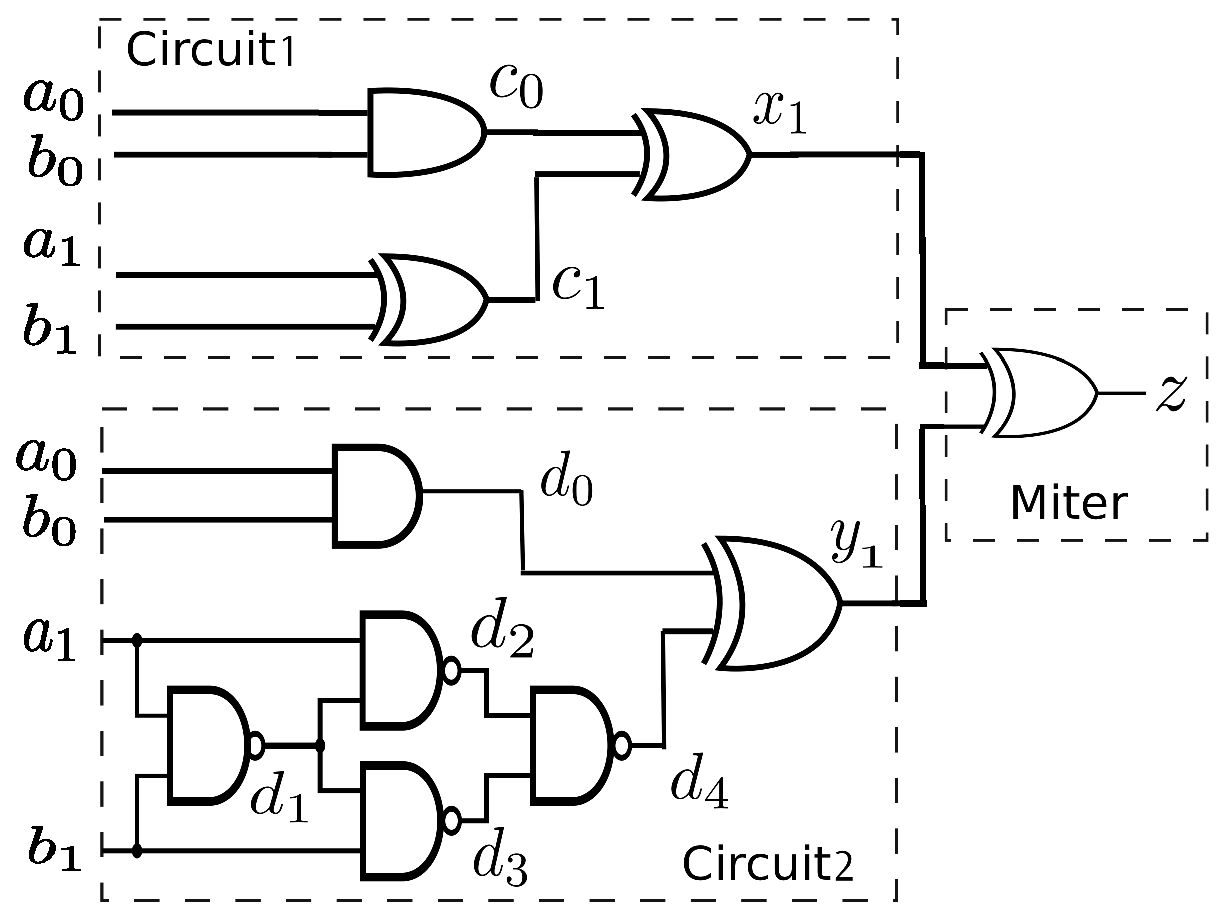
\includegraphics[scale=0.40]{./figures/1bitmiter.eps}
%}
%\caption{Miter}
%\label{fig:1bitmiter}
%\end{figure}

%The above two circuits are functiaonally equivalent and their polynomials are described as follows:


%\begin{eqnarray}
 %\left .  \begin{aligned}
	%& c_0 + a_0\cdot b_0   \\
	%& c_1 + a_1 + b_1   \\
	%& x_1 + c_0 + c_1   \\
	 %\end{aligned} 
%\ \right\}
 %&\qquad&  \text{\it Circuit $1$: $F_{1}$} \nonumber \\
 %\left . \begin{aligned}
	%&d_0+a_0 \cdot b_0 \\
	%&d_1+a_1\cdot b_1+1   \\
	%&d_2+ a_1\cdot d_1+1   \\
	%&d_3+ b_1\cdot d_1+1  \\
	%&d_4+d_2\cdot d_3			\\
	%&y_1+d_0+ d_4   		\\
 %\end{aligned} 
%\right\}
 %&\qquad&  \text{\it  Circuit $2$}: F_{2}  \\
 %\left .  \begin{aligned}
	%& x_1 + y_1 + 1  			
 %\end{aligned} 
%\right\}
 %&\qquad& \text{Miter $f_{m}$:}X \neq Y \nonumber
%\end{eqnarray}

\begin{Example}\label{exp:1bitmiter}
Let us re-consider Example \ref{exp:wnfail}. Based on our topological
term ordering of the circuit, we impose a {\it lex} term order with: \\  
$ x_1 >  y_1 > d_4 > d_3 > d_2 > d_1> d_0 >c_1 > c_0 > a_0 > a_1 > b_0 > b_1$, \\ 
Then the set of polynomials of the miter circuit
$\{ F_{1},F_{2}, f_{m} \}$ does not constitutes a Gr\"obner
Basis. This is because the miter polynomial $f_m: t X - t Y+1$
and output polynomial $f_X$ of circuit $C_1$, $f_X: X+x_0+x_1\cdot
\alpha$, has a common variable $X$  in their leading terms $tX$
and $X$, respectively. Therefore, $lt(f_m)$ and $lt(f_o)$ are not
relatively prime. Moreover, $Spoly(f_m,f_X)$ $\stackrel{F_1, F_2,
  f_m}{\longrightarrow} r$, $r\neq 0$, thus violating the property of
a Gr\"obner basis that all S-polynomials should reduce to zero. 
\end{Example}

This suggests that we may have to compute a reduced Gr\"obner
basis. However, in the next section, we describe our results that can
identify {\it a minimum number of S-polynomial computations} that are
sufficient and necessary to prove equivalence or to detect bugs. 

%%%%%%%%%%%%%%%%%%%%%%%%%%%%%%%%%%%%%%%%%%%%%%%%%%%%%%%%%%%%%%%%%%%%
%%%%%%%%%%%%%%%%%%%%%%%%%%%%%%%%%%%%%%%%%%%%%%%%%%%%%%%%%%%%%%%%%%%%
%%%%%%%%%%%%%%%%%%%%%%%%%%%%%%%%%%%%%%%%%%%%%%%%%%%%%%%%%%%%%%%%%%%%
\section{Verification Using a Minimal Number of S-polynomial Computation}


% Let $F_1, F_2$ represent polynomials generated from circuit $C_1$ and
% $C2$ respectively. Let $f_m$ represent the miter polynomial.
% Let $F=\{F_1,F_2,f_m\}=\{f_1,f_2,\ldots,f_s, f_m\}$ denote this set of
% polynomials derived from the miter circuit.  Let $\{x_1,\dots,x_d\}$
% denote all variables occurring in $F$. Let $J = \langle
% F_1,F_2,f_m\rangle \subset \mathbb{F}_{2^k}[x_{1},\dots,x_{d}]$ denote
% the ideal generated by these polynomials. Let $f_o \in F$ denote the
% only polynomial such that $lt(f_o)$ and $lt(f_m)$ are not relatively
% prime.  

% Based on our term order, such polynomials $f_o, f_m \in F$ always
% exist. Polynomial $f_o \neq f_m$ corresponds to the output of circuit
% $C1$ or $C_2$. Moreover, the leading term of miter polynomial $f_{m}$
% always corresponds to the output of either circuit $C_1$ or $C2$. 
% Let $T=\{x_1,\dots,x_d\}$ denote all variables occurring in $F$, of
% which, let $T_{PI} \subset T$ denote the set of primary inputs. 

% To derive a minimum number of S-polynomial computations for our
% problem,  we first consider a pair of polynomials that are not
% relatively prime: $f_{m}$ and $f_{o}$. In Example \ref{exp:wnfail},
% $f_o=X+x_0+x_1\cdot \alpha$ and $f_m=t\cdot X-t\cdot Y+1$.  Because of
% the existence of $f_{m}$ and $f_{o}$, $\{F_1,F_2,f_m\}$ does not
% constitute a Gr\"obner basis.  


% Therefore, to claim that $f_{m}$ and $f_{o}$ is the only pair of polynomials that needs to be reduced in Gr\"obner basis computation
% of $\{ F \}$, we have the following lemma and theorem: 

To identify a minimum number of S-polynomial computations in
Buchberger's algorithm, we will make use of the following lemma. 
\begin{Lemma}\label{lem:root}
Let $r \in \mathbb{F}_2[x_1, \dots, x_d]$ be a multi-linear polynomial
expression; i.e. r is a nonconstant polynomial such that every
monomial term in $r$ contains variables of degree $1$. Then $r$ has a
root in $\mathbb{F}_2^d$. 
\end{Lemma}

\begin{Proof}
Let $l(r)$ denote the number of nonzero monomials appearing in $r$. We
will perform induction on $l(r)$. Note that in $\mathbb{F}_2$,
the coefficient of all non-zero monomials is 1.

The case $l(r)=1$ is trivial, as $r = x_1x_2\dots x_t$, for some $t
\leq d$. A polynomial with one monomial term always has a solution. 

For the general case, $l(r) \geq 2$. Then  we can always write $r =
r' + M$ where $M$ is a product of monomials. After appropriately
re-labeling the variables, we can assume that $x_1$ divides $M$,
i.e. $x_1$ appears in $M$. If $x_1$ divides $r'$ too, then $x_1$
divides $r$ as well. As a consequence, we obtain $x_1=0$ as a
solution for $r=0$. So, $r$ has a root in $\mathbb{F}_2$. 

If $x_1$ does not divide $r$, then it does not divide $r'$. So
variable $x_1$ does not appear in $r'$. Then, let $r"=\mathcal{F}(0,
x_2,\ldots, x_d)$. Note that $l(r") < l(r)$, as monomial $M$ does not
appear in $r"$. By induction, there is a solution $(x_2, \dots, x_d)$
for $r"=0$, which also gives a solution $(0, x_2, \ldots, x_d)$ for
$r$.  Thus $r$ always has a root in $F_2$.
\end{Proof}

Now we state and prove the following theorem.

\begin{Theorem}\label{thm:miter}
Let $F_1, F_2$ correspond to the set of polynomials
derived from circuits $C_1, C_2$, respectively. Let $f_m$ be the miter
polynomial. Let $F = \{F_1, F_2, f_m\}$ and $J=\langle F \rangle
\subset \mathbb{F}_{2^k}[x_{1},\dots,x_{d}]$ be the ideal of
polynomial corresponding to the miter circuit. Impose the circuit
topology-based monomial order $>$ from Proposition
\ref{prop:top-order}. Let $F_0 = \{ x_1^{2^k} - x_1, \dots,
x_d^{2^k} - x_d\}$ be the vanishing polynomials of $\mathbb{F}_{2^k}$;
and $J_0 = \langle F_0 \rangle$. Let $f_o \in F$ ($f_o \neq f_m$)
be the only polynomial such that  the leading terms of $f_m, f_o$ are
not relatively prime. Then $V_{\mathbb{F}_{2^k}}(J)=\emptyset \iff
r=1$, where $r$ is computed as  $Spoly(f_m, f_o)$
$\stackrel{F,F_0}{\longrightarrow}_+ r$. 

\end{Theorem}

\begin{Proof}
Let $q=2^k$, and let $G$ and $G_{red}$, respectively, denote the
Gr\"obner basis and the reduced Gr\"obner basis of $(J + J_0)$. Let
$T$ represent the set of all variables  occurring in $F$, and let
$T_{pi} \subset T$ denote the set of all primary inputs.   

Our objective is to deduce whether or not the variety
$V_{\mathbb{F}_{2^k}}(J)=\emptyset$, {\it without actually computing a
reduced Gr\"obner basis}. Recall, according to Theorem \ref{wnull:ff}, 
$V_{\mathbb{F}_{q}}(J)=\emptyset \iff G_{red}=\{1\}$, so we
only need to check whether $G_{red} =\{1\}$? Based on our term
ordering, we will try to identify the polynomials that constitute
$G_{red}$. 

% We claim that $GB(J+J_{0})=\{F,F_{0},r\}$, where $r$ is given
% above. In other words, $r$ is the only polynomial that will be
% generated in Buchberger's algorithm.

%This can be shown as follows: 
In the first iteration of Buchberger's
algorithm, $Spoly(f_m,f_o)$ is the only polynomial that needs to be
computed and reduced to obtain $r$, as all other S-polynomials reduce
to zero, due to Theorem \ref{thm:contrib}. We need to consider three
cases: 

\begin{itemize}
\item Case 1: $r = 1$.
\item Case 2: $r = 0$.
\item Case 3: $r$ is a  non-constant multi-linear polynomial
  consisting of only primary input variables of the circuit.
\end{itemize}

{\bf Case 1} is the trivial case: If $r = 1$, then $1\in G$, so
$G_{red} = \{1\}$ and therefore $V(J + J_0) = \emptyset$. The
miter is infeasible and the circuits are equivalent.

{\bf Case 2}: When $r = 0$, no new polynomial is created in
Buchberger's algorithm. Therefore $G = \{F, F_0\}$.
While the set $\{F, F_0\}$ is itself a Gr\"obner basis, it is not
reduced. So, what is the reduced basis $G_{red}$? We will show that
$G_{red} \neq \{1\}$ and this will imply that $V(J + J_0) \neq
\emptyset$.  

To reduce a Gr\"obner basis $G$, we take all polynomials $f \in G$ and
reduce $f\stackrel{G - f}{\longrightarrow}_+ f'$. All such $f'$
constitute $G_{red}$. We will consider such a reduction for $G = \{F,
F_0\}$. For all $f_j \in F$, let $f_j = x_j +P_j$, where 
$P_j = \text{tail}(f_j)$ and $lm(f_j)=x_j$ where $x_j \notin
T_{pi}$. This is due to our term order where only gate outputs ($x_j$)
appear as leading terms of all polynomials. Let $v$ be any variable
in $P_j$. If $v\in \{T-T_{pi}\}$ (non-primary-input), then $v=lm(f_k)$ 
($k\neq j$).  Thus $f_j \xrightarrow{ \{F,F_0\}-f_j }{f_j^{'}}$, where
$f_j^{'}=x_j+P_j^{'}$.  In such a case, $P_j^{'}$ contains only
primary inputs.  From a circuit-structure perspective,
this reflects that any internal gate output $x_j$ can be expressed in
terms of primary inputs.

Similarly, $x_i^{q}-x_i$ with $x_i\in \{T-T_{pi}\}$
will reduce to zero, and only vanishing polynomials of primary inputs
will remain in $F_0$. Moreover, since circuit inputs are bit-level,
$x_{pi}^2 = x_{pi}$; so $x_{pi}^{2}-x_{pi}$, $x_{pi}\in \{T_{pi}\}$,
are the vanishing polynomials remaining in the reduced basis. Let
$F^{'}=\{x_j+P_j^{'}\}$, where $x_j \in T$. Then, the reduced
Gr\"obner basis $G_{red}$ of $\{F, F_0\}$ = $reducedGB(\{F\} \cup
\{x_i^{q}-x_i\})=\{F^{'}\} \cup \{x_{pi}^{2}-x_{pi}\}$. Clearly,
$G_{red} \neq 1$. We conclude, if $r=0$, $G_{red} \neq \{1\}$, and
$V(J + J_0) \neq \emptyset$. The miter constraints are feasible and the
circuits are not equivalent. 


{\bf Case 3}: If $r$ is a non-constant polynomial, then due to our
term order and Corollary \ref{thm:mini}, $r$ will contain only the
primary input variables of the circuit. Moreover, as these variables
are Boolean, $x_{pi}^2 = x_{pi}^3 = \dots = x_{pi}$, all variables in
the monomials of $r$ have degree 1, and $r$ is multi-linear.

% In such a case, according to
% the proof in Theorem \ref{thm:contrib}, $Spoly(r,x_{pi}^{q}-x_{pi})
% \stackrel{G}\rightarrow _+0$, where $x_{pi}$ is a primary
% input. Therefore, for both cases in Step 1, 
% there are no new polynomials generated.

% With the knowledge of $GB(J+J_{0})=\{J,J_{0},r\}$, we can deduce what
% the $redGB(J+J_{0})$ is now. 


%The last case is when $r \neq 0$, what is $redGB(J+J_{0})$? 

%Recall that $lm(r)$ can merely contain primary inputs and is a
%multi-linear polynomial.  
After the first iteration of Buchberger's algorithm, we obtain $\{F,
F_0, r\}$ in the basis. Because $r$ contains only primary inputs,
$lt(r)$ is relatively prime w.r.t. leading terms of all polynomials in
$F$. So the Gr\"obner basis of $\{F,r\}$ is $\{F,r\}$ itself.

However, $\{F,r\}\cup \{F_{0}\}$ is {\it not} a Gr\"obner basis,
because $lm(r)$ and $lm(x_k^{q}-x_k)$ are not relatively prime when
$x_k\in T_{pi}$.  Therefore, $G = GB(\{F,r\}\cup
\{F_{0}\}) = \{F\} \cup GB(r\cup \{F_{0}\})$. In such a
case, if we can show that $1 \notin GB(r\cup \{F_{0}\})$, then
$1\notin GB(\{F,F_{0},r\})$. 

To show $1 \notin GB(r\cup \{F_{0}\})$, we utilize the Weak
Nullstellensatz Theorem \ref{wnull:ff}: if $V(r\cup \{F_{0}\})\neq
\emptyset$,  then $1 \notin GB(r\cup \{F_{0}\})$. In Lemma
\ref{lem:root}, we showed that if $r$ is a multi-linear  
polynomial, it always has a root. This means that $V(r\cup
\{F_{0}\})\neq \emptyset$.  Therefore $1 \notin GB(r\cup
\{F_{0}\})$. This proves Case 3: if $r$ is not 0 or 1, then $\{1\}
\notin G = GB(F,F_0)$.  

So, we conclude that:
\begin{equation}
	V_{\mathbb{F}_{2^k}}(J)=\emptyset \iff r=1.
\end{equation}
\end{Proof}

Combining with Corollary \ref{thm:mini}, the above theorem can be
re-stated based on a minimal Gr\"obner basis. 
\begin{Corollary}\label{cor:miter}
Let $J=\langle F \rangle \subset \mathbb{F}_{2^k}[x_{1},\dots,x_{d}]$ 
on which we impose our circuit-based monomial order $>$.
Let $J_0^{PI}=\langle x_{pi}^{2}-x_{pi}\rangle$, where $x_{pi}\in PI$.
Let $f_o, f_m$ be the only polynomial pair such that $lm(f_m),
lm(f_o)$ are not relatively prime. Then
$V_{\mathbb{F}_{2^k}}(J)=\emptyset \iff r=1$, where $r$ is computed as
$Spoly(f_m,f_o) \stackrel{J,J_0^{PI}}{\longrightarrow}_+ r$.

\end{Corollary}

Theorem \ref{thm:miter} and Corollary \ref{cor:miter} provide the
foundation of our verification formulation. We only need one
S-polynomial computation to identify whether or not the two circuits
are equivalent. Our overall approach is described in the following
algorithm. 


\begin{algorithm}[hbt]
\SetAlgoNoLine

 \KwIn{Two Circuit Implementations with outputs $X$ and $Y$ (Boolean equations).}
 \KwOut{$1$ if $X=Y$. Bug polynomial $r$ if $X\neq Y$.}
%%%%%%%%%%%%%%%%%%%%
%%%%%%%%%%%%%%%%%%%%

\For { (i=0; i $<$ number of eqns; i++) }
  	{
  		\CommentSty{/*Each equation is transformed to polynomials */\;}
  		poly[i] = Eqn-to-Poly(eqn[i])\;
  		\CommentSty{/*Each equation is transformed to sum-of-term*/\;}
  		newpoly[i] = Sum-of-term(poly[i])\;
	}
%%%%%%%%%%%%%%%%%%%%
\CommentSty{/*Obtain circuit-based variable order*/\;}
ordered\_var=T\_Traversal(newpoly)\;
%%%%%%%%%%%%%%%%%%%%
\For {x $\in$ \{PI\} }
	{
		\CommentSty{/*append vanishing polynomials*/\;}
    	vanpoly[i]=$x^2+x$\;
	}    
\CommentSty{/*Identify polynomials that need to be reduced*/\;}	
{$f_{o}$, $f_{m}$}=Identify(newpoly, vanpoly)\;
To\_Be\_Reduced=Spoly($f_{o}$, $f_{m}$)\;
r=reduce(To\_Be\_Reduced, vanpoly, ordered\_var)\;
\eIf {r=\{1\}}
   {
   	 return $1$;
   }
   {
   	 return Bug polynomial $r$; %Bug polynomial;
   }	 

\caption{Our Proposed Equivalence Checking Algorithm}\label{alg:ecall}
\end{algorithm}


Algorithm \ref{alg:overall} first inputs the Boolean expressions of
the given circuit implementation. Each expression is then transformed
into polynomials $F$ using the mappings shown in Equation
\ref{b2poly}. All polynomials are then normalized into a sum-of-term
form using the distributive law $A(B+C)=AB+AC$.  
Then we perform a reverse topology traversal of the circuit to
derive our  variable and ordering. Then, we append vanishing
polynomials $F_{0} =\{x^2 + x \}$ for all $x \in$ primary inputs.  
Subsequently, we identify the two polynomials $f_{m}$ and $f_{o}$ that
have common variables in their leading terms. Finally, we conduct a
polynomial reduction of $Spoly(f_{m},f_{o})$  modulo $\{F \cup F_{0}\}$.  
If the reduction result is $r = 1$, the two circuits are equivalent. 
If $r \neq 1$, the circuits are not equivalent. Again, any assignment
to the variables that make $r \neq 1$ provides an input vector that
can be used as a counter-example for debugging. 

%%%%%%%%%%%%%%%%%%%%%%%%%%%%%%%%%%%%%%%%%%%%%%%%%%%%%%%
%%%%%%%%%%%%%%%%%%%%%%%%%%%%%%%%%%%%%%%%%%%%%%%%%%%%%%%
%%%%%%%%%%%%%%%%%%%%%%%%%%%%%%%%%%%%%%%%%%%%%%%%%%%%%%%
\section{Improving Polynomial Reduction using $F_4$-style reduction}

Through the results described above, the need for Buchberger's
algorithm is obviated and verification can be performed by analyzing
the result of just one S-polynomial reduction. Therefore, the most
intensive computational step is that of polynomial division 
$Spoly(f_m,f_o) \stackrel{F,F_0}{\longrightarrow}_+ r$. When the two
circuits $C_1, C_2$ are very large, the polynomial set $\{F, F_0\}$
also becomes extremely large. This division procedure then becomes the
bottleneck in verifying the equivalence. To further improve upon our 
approach, we exploit the relatively recent concept of $F_4$-style
polynomial reduction \cite{f4}, which implements polynomial division
using successive row-reductions on a matrix. 



% As described in Algorithm \ref{alg:overall}, polynomial reduction is
% the most time consuming step.  Therefore, to improve the efficiency of
% polynomial reduction,  polynomial reduction can be formulated as a
% matrix operation as used in $F4$ \cite{f4} that is a variant of
% Buchberger's algorithm.  In particular, polynomial reduction is
% formulated as row-reductions of a single matrix in $F4$. 

% However, the approach in \cite{f4} is applied for general purpose
% polynomial reduction and cannot achieve the best  performance for our
% problem.  Therefore, we need suitably engineer the $F4$-style
% reduction to better enhance our approach. 

Let us first describe the matrix representation for polynomial algebra
operations. 


{\bf Matrix representation of polynomials:} Each row $i$ of the matrix
$M$ corresponds to polynomial $f_i$, whereas each column $j$
corresponds to monomial $m_j$.
% of $f_i$corresponds to column $j$. 
If the $j^{th}$ entry on row $i$ in matrix is $1$, i.e. $M(i, j) = 1$,
it means the $j^{th}$ monomial is present in the $i^{th}$ polynomial.
Similarly, $M(i, j) = 0$ denotes the absence of $m_j$ in $f_i$. 
Since we are operating in $\mathbb{F}_{2^k}$, coefficients
are always $\{0, 1\}$, and no specific representation of coefficients
is required. Note, however, that the entries in rows and columns have
to satisfy the imposed term ordering. 
 
\begin{Example}
Given two polynomials: $f_{1}=a_{0}+a_{1}\cdot b_{1}+1$ and
$f_{2}=a_{0}\cdot b_{0}+b_{1}+1$ with term ordering {\it lex} with
$a_{0}>a_{1}>b_{0}>b_{1}$.  First, we sort all monomials occurring in
$f_{1}$ and $f_{2}$ w.r.t. term ordering: $a_{0}\cdot b_{0}
>a_{0}>a_{1}\cdot b_{1}> b_{1}>1$. 

Then, we associate these sorted monomials with the columns of the
matrix. The polynomials are also sorted according to the term order
before they are associated with the rows of the matrix. For example,
since $lm(f_{2})>lm(f_{1})$, $f_{2}$ appears on row $1$ and $f_{1}$
appears on row $2$. 
%(Actually $F4$ does not require such a polynomial ordering. 
The generated matrix is shown in Table \ref{tab:matrix}. 

	\begin{table}[htb]
	\begin{center}
	\caption{Matrix representation for polynomials.}
	\label{tab:matrix}
	\begin{tabular}{|c|c|c|c|c|c|} \hline 
			&$a_{0}\cdot b_{0}$  	&$a_{0}$ 	&$a_{1}\cdot b_{1}$		&$b_{1}$ 	&$1$  \\
	\hline 
	$f_{2}$ & 1 &0 & 0 & 1 & 1 \\
	\hline
	$f_{1}$ & 0 &1 & 1 & 0 & 1 \\
	\hline
	\end{tabular}
	\end{center}
	\end{table}
\end{Example}	


Polynomial reduction requires operations of addition/subtraction and
cancellation of leading terms. We demonstrate how the
addition/subtraction and division operations are implemented on

{\bf Matrix subtraction for polynomials:} The subtraction of two
polynomials can be formulated as a row-eduction in the matrix. Since
coefficients of polynomials are computed (mod $2$) in our case,
row-reductions are also performed (mod $2$). 
%	which is another difference from $F4$-style reduction.
	
\begin{Example}	
	Again consider $f_{1}=a_{0}+a_{1}\cdot b_{1}+1$ and
        $f_{2}=a_{0}\cdot b_{0}+b_{1}+1$ with {\it lex} order:
        $a_{0}>a_{1}>b_{0}>b_{1}$. 
	Let us perform $f_{1}-f_{2}$: % the polynomial form is: 
	$f_{1}-f_{2}=f_{2}-f_{1} \pmod 2=a_{0}\cdot b_{0}+a_{0}+a_{1}\cdot b_{1}+b_{1}$.
	On the matrix, each entry on row $2$ is subtracted from %subtracts
        the corresponding entry on row $1$ and the result is stored in row
        $2$, as shown in Table \ref{tab:subtract}.
	
	 \begin{table}[h!]
	\begin{center}
	\caption{Matrix subtraction of polynomials.}
	\label{tab:subtract}
	\begin{tabular}{|c|c|c|c|c|c|} \hline 
			& $a_{0}\cdot b_{0}$  & $a_{0}$ & $a_{1}\cdot b_{1}$ & $b_{1}$ & $1$  \\
	\hline 
	$f_{2}$ & 1 &0 & 0 & 1 & 1 \\
	\hline
	$f_2 - f_{1}$ & 1 &1 & 1 & 1 & 0 \\
	\hline
	\end{tabular}
	\end{center}
	\end{table}
	
\end{Example}

{\bf Matrix reduction for polynomials:} Polynomial
division is implemented as cancellation of leading terms. The
reduction step in Algorithm \ref{alg:polydiv} that cancels leading
terms is:   
\begin{equation}\label{eqn:mat-red}
	{f_1}/{f_2}=f_{1}-\frac{lm(f_1)}{lm(f_2)}\cdot f_{2} 
\end{equation}
 
In matrix representation, 
%instead of creating two rows for $f_{1}$ and $f_{2}$, 
we create two rows, one each for $f_{1}$ and $\frac{lm(f_1)}{lm(f_2)}\cdot f_{2}$,
and then perform subtraction on the matrix; this is shown in Example
\ref{exp:division}.  
 
\begin{Example}\label{exp:division}
Given two polynomials: $f_{1}=a_{0}\cdot b_{1}+a_{0}+1$ and
$f_{2}=a_{0}+1$ with term order {\it lex}:
$a_{0}>a_{1}>b_{0}>b_{1}$. Consider the polynomial reduction:

\begin{equation}
{f_1}/{f_2}=f_{1}-\frac{a_{0}\cdot b_{1}}{a_{0}}\cdot f_{2} =f_{1}-b_{1}\cdot f_{2} \nonumber
\end{equation}
	 
We create two rows in matrix for $f_{1}$ and $b_{1}\cdot f_{2}$ and
insert monomials from $f_{1}$ and $b_{1}\cdot f_{2}$ into the matrix
columns, as shown in Table \ref{tab:red}.  
	 
	\begin{table}[htb]
	\begin{center}
	\caption{ Step 1 of matrix reduction for polynomials: representation.}
	\label{tab:red}
	\begin{tabular}{|c|c|c|c|c|} \hline 
			&$a_{0} \cdot b_{1}$ & $a_{0}$ & $b_{1}$ & $1$  \\
	\hline 
	$b_{1}\cdot f_{2}$ & 1 &0 & 1  & 0 \\ 
	\hline
	$f_{1}$ & 1 &1 & 0 & 1  \\
	\hline
	\end{tabular}
	\end{center}
	\end{table}
	
	Then we conduct $f_{1}-b_{1}\cdot f_{2}$:
	
	\begin{table}[htb]
	\begin{center}
	\caption{Step 1 of matrix reduction for polynomials: subtraction.}
	\label{tab:red2}
	\begin{tabular}{|c|c|c|c|c|} \hline 
			&$a_{0} \cdot b_{1}$ & $a_{0}$ & $b_{1}$ & $1$  \\
	\hline 
	$b_{1}\cdot f_{2}$ & 1 &0 & 1  & 0 \\ 
	\hline
	$f_{1} - b f_2$ & 0 &1 & 1 & 1  \\
	\hline
	\end{tabular}
	\end{center}
	\end{table}
	
	Finally, row $2$ represents the reduction result of ${f_1}/{f_2}=a_{0}+b_{1}+1$.
	
 \end{Example}

With the above basic polynomial operations formulated as matrix
operations, we now describe our algorithm to create the matrix of
polynomials corresponding to our verification instance (miter
circuit). The algorithm is shown in Algorithm \ref{alg:matrix}. The
main idea behind this algorithm is to setup the rows  of
the matrix (polynomials) in a way that polynomial division can be
subsequently performed by subtracting row $i$ from row $i-1$. In the
algorithm, the computation $L:=L \cup \frac{mon}{lm(f_{k})}\cdot
f_{k}$ in the while-loop, actually corresponds to  
$\frac{lm(f_1)}{lm(f_2)}\cdot f_{2} $ in
Equation \label{eqn:mat-red}. 


\begin{algorithm}[hbt]
\SetAlgoNoLine

 \KwIn{$f, F=\{f_1,\dots,f_s$\} with $f_{1}>f_{2}>\dots>f_{s}$. }
 \KwOut{A matrix representing $f \xrightarrow{f_1,\dots,f_s}_+r$}
  %%%%%%%%%%%%%%%%%%%%
	\CommentSty{/*Let $L$ be the set of polynomials corresponding to rows of matrix*/\;}
	L:=\{f\} \;{}
	\CommentSty{/*The index of polynomials in $F$*/\;}
	i:=1\;
%	\CommentSty{/*Initial remainder $r$ is set as $f$*/\;}
%	r:=f\;
	\CommentSty{/*Let $M_{L}$ be the set of monomials */\;}
	$M_{L}$:=\{ monomials of f\} \;{}
%	\CommentSty{/*Let $Done$ be the set of monomials that have been handled*/\;}
%	$Done:=\{\}$\;
%	\CommentSty{/*The first $i-1$ monomials of $M_{L}$ have been handled*/\;}
	mon:= the $i^{th}$ monomial of $M_{L}$\;
	\While { mon $\notin PrimaryInputs$ }
		{
			Identify $f_{k} \in F$ satisfying: $lm(f_{k})$ can divide $mon$ \;
			\CommentSty{/*add new polynomial to L as a new row in matrix*/\;}
			$L:=L \cup \frac{mon}{lm(f_{k})}\cdot f_{k}$ \;
			\CommentSty{/*Add monomials to $M_{L}$ as new columns in matrix */\;}
			$M_{L}$:=$M_{L} \cup \{ \text{monomials of } \frac{mon}{lm(f_{k})}\cdot f_{k}\}$ \;{}
			%\CommentSty{/*Cancel adjacent monomials if they are the same*/\;}
			%CancelAdjMons($M_{L}$)\;
			$i:=i+1$\;{}
			mon:= the $i^{th}$ monomial of $M_{L}$\;
		}
\caption{Generating the Matrix for Polynomial Reduction}\label{alg:matrix}
\end{algorithm}

%The above algorithm is actually a simulation of polynomial reduction. 

To better understand the algorithm, we describe the matrix
construction procedure in Example \ref{exp:consmatix}. 

\begin{Example}\label{exp:consmatix}
	Suppose that two functionally equivalent circuits and the
        miter are  represented by the following polynomials at
        bit-level (i.e. over $\mathbb{F}_2$):
	\begin{eqnarray}
		f_m&=&x+y+1, \nonumber \\
		f_o&=&x+n_0+n_2, \nonumber \\
		f_1&=&y+n_{10}, \nonumber \\
		f_2&=&n_0+i_2\cdot i_3, \nonumber \\
		f_3&=&n_2+i_0\cdot i_1, \nonumber \\
		f_4&=&n_{10}+n_7, \nonumber \\
		f_{5}&=&n_7+n_6+n_4\cdot i_0, \nonumber \\
		f_{6}&=&n_6+n_5+n_3\cdot i_1, \nonumber \\
		f_{7}&=&n_5+n_4\cdot n_3,  \nonumber \\
		f_{8}&=&n_4+i_1+i_3, \nonumber \\
		f_{9}&=&n_3+i_0+i_2;\nonumber 
	\end{eqnarray}
	
        Note that $i_0, \dots, i_3$ denote the primary inputs of the
        circuits. The circuit topology-based monomial order is derived
        as {\it lex} with
        $x>y>n_0>n_2>n_{10}>n_7>n_6>n_5>n_4>n_3>i_0>i_1>i_2>i_3$. 
	All polynomials above have already been sorted (ordered) according to their
        leading terms in descending order. All monomials in each
        polynomial are also ordered. 
	
	In this case, $f=Spoly(f_{m},f_{o})=y+n_0+n_2+1$ and
        $F=\{f_{1},\dots, f_{9}\}$.  We want to show the algorithm's
        operation to construct a matrix for the reduction $f
        \xrightarrow{F}_{+}r$.  
	
		
	{\it Initialization:}
	\begin{eqnarray}
		L&:=&\{f\}; \nonumber \\
		M_{L}&:=&\{ y,n_0,n_2,n_{10},1\}; \nonumber \\
		mon&:=& y ;\nonumber
	\end{eqnarray}\\
	
	{\it Iteration $i=1$:}	
	\begin{eqnarray}
		f_{k}&:=&f_{1}=y+n_{10}; \nonumber \\
		L&:=&\{f,f_1\}; \nonumber \\
		M_{L}&:=&\{ y,n_0,n_2,n_{10},1\}; \nonumber \\
		i&:=&2;  \nonumber \\
		mon&:=& n_0\nonumber 
	\end{eqnarray}\\
	
	{\it Iteration $i=2$:}
	\begin{eqnarray}
		f_{k}&:=&f_{2}=n_0+i_2\cdot i_3; \nonumber \\
		L&:=&\{f,f_1,f_{2}\}; \nonumber \\
		M_{L}&:=&\{ y,n_0,n_2,n_{10},i_2 \cdot i_3,1\}; \nonumber \\
		i&:=&3;  \nonumber \\
		mon&:=& n_2\nonumber 
	\end{eqnarray}\\
	
	{\it Iteration $i=3$:}
	\begin{eqnarray}
		f_{k}&:=&f_{3}=n_2+i_0\cdot i_1; \nonumber \\
		L&:=&\{f,f_1,f_{2},f_{3}\}; \nonumber \\
		M_{L}&:=&\{ y,n_0,n_2,n_{10},i_0 \cdot i_1,i_2 \cdot i_3,1\}; \nonumber \\
		i&:=&4;  \nonumber \\
		mon&:=& n_{10}\nonumber 
	\end{eqnarray}\\

	{\it Iteration $i=4$:}
	\begin{eqnarray}
		f_{k}&:=&f_{4}=n_{10}+n_7; \nonumber \\
		L&:=&\{f,f_1,f_{2},f_{3},f_{4}\}; \nonumber \\
		M_{L}&:=&\{ y,n_0,n_2,n_{10},n_7,i_0\cdot i_1,i_2\cdot i_3,1\}; \nonumber \\
		i&:=&5;  \nonumber \\
		mon&:=& n_7\nonumber 
	\end{eqnarray}\\
	
	
	{\it Iteration $i=5$:}
	\begin{eqnarray}
		f_{k}&:=&f_{5}=n_7+n_6+n_4\cdot i_0; \nonumber \\
		L&:=&\{f,f_1,f_{2},f_{3},f_{4},f_{5}\}; \nonumber \\
		M_{L}&:=&\{ y,n_0,n_2,n_{10},n_7,n_6,n_4\cdot i_0,i_0\cdot i_1,i_2\cdot i_3,1\}; \nonumber \\
		i&:=&6;  \nonumber \\
		mon&:=& n_6\nonumber 
	\end{eqnarray}\\
	
	{\it Iteration $i=6$:}
	\begin{eqnarray}
		f_{k}&:=&f_{6}=n_6+n_5+n_3\cdot i_1; \nonumber \\
		L&:=&\{ f,f_1,f_{2},f_{3},f_{4},f_{5},f_{6}\}; \nonumber \\
		M_{L}&:=&\{ y,n_0,n_2,n_{10},n_7,n_6,n_5,n_4\cdot i_0,n_3\cdot i_1,i_0\cdot i_1,i_2\cdot i_3,1\}; \nonumber \\
		i&:=&7;  \nonumber \\
		mon&:=& n_5\nonumber 
	\end{eqnarray}\\
	
	{\it Iteration $i=7$:}
	\begin{eqnarray}
		f_{k}&:=&f_{7}=n_5+n_4\cdot n_3; \nonumber \\
		L&:=&\{ f,f_1,f_{2},f_{3},f_{4},f_{5},f_{6},f_{7}\}; \nonumber \\
		M_{L}&:=&\{ y,n_0,n_2,n_{10},n_7,n_6,n_5,n_4\cdot n_3,n_4\cdot i_0,n_3\cdot i_1,i_0\cdot i_1,i_2\cdot i_3,1 \}; \nonumber \\
		i&:=&8;  \nonumber \\
		mon&:=& n_4\cdot n_3 \nonumber 
	\end{eqnarray}\\
	
	{\it Iteration $i=8$:}
	\begin{eqnarray}
		f_{k}&:=&f_{8}=n_4+i_1+i_3; \nonumber \\
		L&:=&\{ f,f_1,f_{2},f_{3},f_{4},f_{5},f_{6},f_{7},n_3 \cdot f_{8}\}; \nonumber \\
		M_{L}&:=&\{ y,n_0,n_2,n_{10},n_7,n_6,n_5,n_4\cdot n_3,n_4\cdot i_0,n_3\cdot i_1,n_3\cdot i_3,i_0\cdot i_1,i_2\cdot i_3,1 \}; \nonumber \\
		i&:=&9;  \nonumber \\
		mon&:=& n_4\cdot i_0\nonumber 
	\end{eqnarray}\\
	
	{\it Iteration $i=9$:}
	\begin{eqnarray}
		f_{k}&:=&f_{8}=n_4+i_1+i_3; \nonumber \\
		L&:=&\{ f,f_1,f_{2},f_{3},f_{4},f_{5},f_{6},f_{7},n_3 \cdot f_8, i_0 \cdot f_8\}; \nonumber \\
		M_{L}&:=&\{ y,n_0,n_2,n_{10},n_7,n_6,n_5,n_4\cdot n_3,n_4\cdot i_0,n_3\cdot i_1,n_3\cdot i_3,i_0\cdot i_1,\nonumber \\
		&{}&i_0\cdot i_3, i_2\cdot i_3,1\}; \nonumber \\
		i&:=&10;  \nonumber \\
		mon&:=& n_3\cdot i_1\nonumber 
	\end{eqnarray}\\
	
	{\it Iteration $i=10$:}
	\begin{eqnarray}
		f_{k}&:=&f_{9}=n_3+i_0+i_2; \nonumber \\
		L&:=&\{ f,f_1,f_{2},f_{3},f_{4},f_{5},f_{6},f_{7},n_3 \cdot f_{8}, i_{0} \cdot f_8,i_1 \cdot f_{9} \}; \nonumber \\
		M_{L}&:=&\{ y,n_0,n_2,n_{10},n_7,n_6,n_5,n_4\cdot n_3,n_4\cdot i_0,n_3\cdot i_1,n_3\cdot i_3,i_0\cdot i_1,  \nonumber \\
		&{}&i_0\cdot i_3, i_1\cdot i_2,i_2\cdot i_3,1\}; \nonumber \\
		i&:=&11;  \nonumber \\
		mon&:=& n_3\cdot i_3\nonumber 
	\end{eqnarray}\\
	
	{\it Iteration $i=11$:}
	\begin{eqnarray}
		f_{k}&:=&f_{9}=n_3+i_0+i_2; \nonumber \\
		L&:=&\{ f,f_1,f_{2},f_{3},f_{4},f_{5},f_{6},f_{7},n_3 \cdot f_{8}, i_{0} \cdot f_{8},i_1 \cdot f_{9}, i_3 \cdot f_{9}\}; \nonumber \\
		M_{L}&:=&\{ y,n_0,n_2,n_{10},n_7,n_6,n_5,n_4\cdot n_3,n_4\cdot i_0, n_3\cdot i_1,n_3\cdot i_3,i_0\cdot i_1,\nonumber \\
		&{}&i_0\cdot i_3, i_1\cdot i_2,i_2\cdot i_3,1\}; \nonumber \\
		i&:=&12;  \nonumber \\
		mon&:=& i_0\cdot i_1 \nonumber 
	\end{eqnarray}\\
	
	{\it Termination:} Because $i_0\cdot i_1$ contains variables
        $\in PrimaryInputs$ only.
	
	Each polynomial in $L$ corresponds to a row in the matrix and
        each monomial corresponds to a column. The generated matrix is
        shown in Table \ref{tab:matrixcons}. 
	
	\begin{sidewaystable} 
	\begin{center}
	\caption{Matrix Created for Polynomial Reduction.} 
	\label{tab:matrixcons}
	\begin{tabular}{|c||c|c|c|c|c|c|c|c|c|c|c|c|c|c|c|c|} \hline 
				&$y$ 	&$n_0$ &$n_2$	&$n_{10}$	 &$n_7$	&$n_6$  &$n_5$   &$n_4\cdot n_3$  &$n_4\cdot i_0$ 	&$n_3\cdot i_1$	&$n_3\cdot i_3$	&$i_0\cdot i_1$		&$i_0\cdot i_3$ 	&$i_1\cdot i_2$	 &$i_2\cdot i_3$   &$1$ \\
		\hline
		$f$   		&1	&1	&1	&0		&0	&0	&0	&0	&0	&0	&0	&0	&0	&0	&0	&1 \\
		\hline
		$f_1$ 		&1	&0	&0	&1		&0	&0	&0	&0	&0	&0	&0	&0	&0	&0	&0	&0 \\
		\hline
		$f_2$ 		&0	&1	&0	&0		&0	&0	&0	&0	&0	&0	&0	&0	&0	&0	&1	&0 \\
		\hline
		$f_3$		&0	&0	&1	&0		&0	&0	&0	&0	&0	&0	&0	&1	&0	&0	&0	&0 \\
		\hline
		$f_4$		&0	&0	&0	&1		&1	&0	&0	&0	&0	&0	&0	&0	&0	&0	&0	&0\\
		\hline{}
		$f_5$		&0	&0	&0	&0		&1	&1	&0	&0	&1	&0	&0	&0	&0	&0	&0	&0\\
		\hline{}
		$f_6$		&0	&0	&0	&0		&0	&1	&1	&0	&0	&1	&0	&0	&0	&0	&0	&0\\
		\hline{}
		$f_7$		&0	&0	&0	&0		&0	&0	&1	&1	&0	&0	&0	&0	&0	&0	&0	&0\\
	\hline{}
$n_3\cdot f_{8}$	&0	&0	&0	&0		&0	&0	&0	&1	&0	&1	&1	&0	&0	&0	&0	&0\\
	\hline{}
$i_0\cdot f_{8}$ 	&0	&0	&0	&0		&0	&0	&0	&0	&1	&0	&0	&1	&1	&0	&0	&0\\
	\hline{}
$i_1 \cdot f_{9}$	&0	&0	&0	&0		&0	&0	&0	&0	&0	&1	&0	&1	&0	&1	&0	&0\\
	\hline{}
$i_3 \cdot f_{9}$	&0	&0	&0	&0		&0	&0	&0	&0	&0	&0	&1	&0	&1	&0	&1	&0\\
	\hline
	\end{tabular}
	\end{center}
	\end{sidewaystable} 
	
	With the generated matrix, the polynomial reduction can be
        formulated as a series of matrix subtractions,  
	i.e., $Row_{i}- Row_{i-1}$. After all row subtractions, the
        reduction result corresponds to the polynomial represented in
        the last row. 

        Two important points to be noted:
	\begin{itemize}
	\item All subtractions are computed modulo $2$.
	\item If polynomials $f_{i}$ and $f_{i-1}$ have no common
          leading monomials, then they cannot conduct a
          reduction. Correspondingly, in the matrix, when conducting
          $Row_{i}- Row_{i-1}$, if the first non-zero entries of
          $Row_{i}$ and $Row_{i-1}$ are not in the same column
          (leading monomials), then we move on to the next row and
          perform $Row_{i+1}-Row_{i-1}$.  
	\end{itemize}

	 This procedure is shown in Table \ref{tab:redres} for $i_1
         \cdot f_{9} - i_0\cdot f_{8}$: here  $lm(i_1 \cdot
         f_{9})=n_{4}\cdot n_{3}$ while $lm(i_0\cdot f_{8})=n_{4}\cdot
         i_0$. These leading monomial are not equal and they cannot
         divide each other. Thus we skip the current row ($i_1 \cdot
         f_{9}$). Instead, we move to the next row ($i_3 \cdot f_{9}$)
         and compute $i_3 \cdot f_{9}-i_0\cdot f_{8}$.   Finally, the
         last entry in Table \ref{tab:redres} corresponds to $r = 1$,
         and that denotes infeasibility of the miter circuit.

	
	\begin{sidewaystable} 
	\begin{center}
	\caption{Matrix Created for Polynomial Reduction.} 
	\label{tab:redres}
	\begin{tabular}[hbt]{|c||c|c|c|c|c|c|c|c|c|c|c|c|c|c|c|c|} \hline 
				&$y$ 	&$n_0$ &$n_2$	&$n_{10}$	 &$n_7$	&$n_6$  &$n_5$   &$n_4\cdot n_3$  &$n_4\cdot i_0$ 	&$n_3\cdot i_1$	&$n_3\cdot i_3$	&$i_0\cdot i_1$		&$i_0\cdot i_3$ 	&$i_1\cdot i_2$	 &$i_2\cdot i_3$   &$1$ \\
		\hline
		$f$   		&1	&1	&1	&0		&0	&0	&0	&0	&0	&0	&0	&0	&0	&0	&0	&1 \\
		\hline
		$f_1$ 		&0	&1	&1	&1		&0	&0	&0	&0	&0	&0	&0	&0	&0	&0	&0	&1 \\
		\hline
		$f_2$ 		&0	&0	&1	&1		&0	&0	&0	&0	&0	&0	&0	&0	&0	&0	&1	&1 \\
		\hline
		$f_3$		&0	&0	&0	&1		&0	&0	&0	&0	&0	&0	&0	&1	&0	&0	&1	&1 \\
		\hline
		$f_4$		&0	&0	&0	&0		&1	&0	&0	&0	&0	&0	&0	&1	&0	&0	&1	&1\\
		\hline{}
		$f_5$		&0	&0	&0	&0		&0	&1	&0	&0	&1	&0	&0	&1	&0	&0	&1	&1\\
		\hline{}
		$f_6$		&0	&0	&0	&0		&0	&0	&1	&0	&1	&1	&0	&1	&0	&0	&1	&1\\
		\hline{}
		$f_7$		&0	&0	&0	&0		&0	&0	&0	&1	&1	&1	&0	&1	&0	&0	&1	&1\\
	\hline{}
$n_3\cdot f_{8}$	&0	&0	&0	&0		&0	&0	&0	&0	&1	&0	&1	&1	&0	&0	&1	&1\\
	\hline{}
$i_0\cdot f_{8}$ 	&0	&0	&0	&0		&0	&0	&0	&0	&0	&0	&1	&0	&1	&0	&1	&1\\
	\hline
$\mathbf{i_1 \cdot f_{9}}$	&$\mathbf{0}$	&$\mathbf{0}$	&$\mathbf{0}$	&$\mathbf{0}$	&$\mathbf{0}$	&$\mathbf{0}$	&$\mathbf{0}$	
&$\mathbf{0}$	&$\mathbf{0}$	&$\mathbf{1}$	&$\mathbf{0}$	&$\mathbf{1}$	&$\mathbf{0}$	&$\mathbf{1}$	&$\mathbf{0}$	&$\mathbf{0}$\\
	\hline
$i_3 \cdot f_{9}$	&0	&0	&0	&0		&0	&0	&0	&0	&0	&0	&0	&0	&0	&0	&0	&1\\
	\hline
	\end{tabular}
	\end{center}
	\end{sidewaystable} 
\end{Example}

% When the matrix representation of our verification problem is
% available, we then send this matrix to GPU  which is highly
% efficient at conducting matrix operations. 

As shown in the above example, the polynomial reduction
result $r$ can be computed by successively subtracting  rows $i$ from
rows $i+1$. Finally, the last row represents $r$. If the last row only
contains the monomial $1$, the two circuits are equivalent. Otherwise, the
polynomial corresponding to the last row represents the bug polynomial. 

%%%%%%%%%%%%%%%%%%%%%%%%%%%%%%%%%%%%%%%%%%%%%%%%
%%%%%%%%%%%%%%%%%%%%%%%%%%%%%%%%%%%%%%%%%%%%%%%%
%%%%%%%%%%%%%%%%%%%%%%%%%%%%%%%%%%%%%%%%%%%%%%%%
\section{Experimental Results}
Our algorithm has been implemented in $C++$ as a high efficient engine for equivalence checking based on computer 
algebra techniques. Our experiments are conducted on a desktop with $2.40$GHz Intel
Core(TM)$2$ Quad CPU and  $8$GB memory running $64$-bit Linux. 

\subsection{Equivalence Checking of Structurally Similar Circuits}
To evaluate the performance of structurally similar circuits, we conduct a equivalence checking
between Mastrovito multiplier and Barrett multiplier (Mastrovito multiplier and Barrett multiplier have similar circuit structures, 
as shown in Chapter \ref{ch:prelim}). Because of the large number of variables and polynomials present in our problem, 
we combine multiple polynomials into one polynomial.
Table \ref{tab:bvsmas} shows the results of verifying Mastrovito multiplier against Barrett multiplier. 
SAT solvers, ABC and CSAT can solve them reasonably fast. Singular can also verify these circuits in seconds.
However, since Singular has a limitation on variable number (not more than $65535$ variables in system),
Singular cannot verify these circuits with size $\ge 96$.
The results also show that our approach is efficient in verifying similar circuits over finite fields and performs
the best among these methods. 

\begin{table}[h!]
\begin{center}
\caption{Verification of Mastrovito multiplier vs. Barrett multiplier. $TO$=$10$hrs. $\star$=Out of variable limitation.
Time is given in seconds.}
\label{tab:bvsmas}
\begin{tabular}{|c||c|c|c|c|c|c|c|} \hline 
Size   			&8  		&16       	&32       	&64      	&96   		&128  		&163		\\
\hline 
\#variables 	&$412$ 		&$1445$ 	&$4587$ 	&$18953$ 	&$42576$ 	&$110543$ 	&$195124$ 	\\
\hline 
\#gates			&$1446$  	&$6846$    	&$25846$   	&$101401$    &$227499$  &$403036$  	&$653021$ 	\\
\hline
MiniSAT   		&$0.02$  	&$0.27$   	&$0.36$  	&$1.60$    	&$17.54$ 	&$5.10$ 	&$28.97$		\\
\hline
PicoSAT   		&$0.02$  	&$0.15$   	&$0.78$  	&$3.90$    	&$6.58$ 	&$41.89$ 	&$130.56$		\\
\hline
PrecoSAT   		&$0.05$  	&$0.40$   	&$1.61$  	&$22.98$   	&$91.90$ 	&$90.25$ 	&$187.53$		\\
\hline
CryptoMiniSAT	&$0.07$  	&$0.82$   	&$1.31$  	&$4.75$    	&$16.81$ 	&$128.22$ 	&$42.78$		\\
\hline
ABC   			&$0.12$  	&$1.07$   	&$0.82$  	&$2.79$    	&$5.72$ 	&$9.79$ 	&$18.67$	\\
\hline
CSAT   			&$0.03$  	&$3.02$   	&$0.58$  	&$0.87$   	&$1.83$ 	&$5.97$ 	&$5.49$		\\
\hline
Singular		&$0.03$  	&$0.17$   	&$0.41$  	&$1.12$   	&$\star$ 	&$\star$ 	&$\star$		\\
\hline
\hline
Our Approach	&$0.00$  	&$0.01$   	&$0.01$  	&$0.02$    &$0.03$  	&$0.05$  	&$0.12$ 	\\
\hline
\end{tabular}
\end{center}
\vspace{-0.2in}
\end{table}


\subsection{Equivalence Checking of Structurally Dissimilar Circuits}
As shown in Table \ref{tab:result}, given two structurally dissimilar circuits (Mastrovito multiplier vs. Montogmery Multiplier), 
SAT/SMT/BDD/AIG is unable to verify the correctness of circuits beyond $16$-bits. 
The reason ABC and C-SAT fail such verification is because structural hashing, utilized by ABC and C-SAT, cannot work on 
structurally dissimilar circuits. In other words, ABC and C-SAT fails to identify the common 
sub-circuits and therefore cannot merge the identical sub-circuits as nodes, which benefits ABC and C-SAT greatly.

Our experiments run verification between Montgomery multiplier, on one hand, and 
 Mastrovito multiplier and Barrett multiplier, on the other hand.
Table \ref{tab:bvsmont} shows the runtime of Barrett multiplier vs. Montgomery multiplier. 
Table \ref{tab:masvsmont} shows the runtime of Mastrovito multiplier vs. Montgomery multiplier. 
Singular stops at verifying $64$ multipliers because of its variable limitation.
In contrast, our approach can successfully verify upto $128$-bit multipliers with dissimilar structures.
Note, verification time for $128$-bit multipliers is significantly less than that of $96$-bit. This result is specially checked and 
therefore it is reliable. The reason lie in the primitive polynomial we choose to construct the circuits. 
Usually if the primitive polynomial itself is simple, then the circuits based on it will have 
less gates than that based on a complex primitive polynomial.


%%%%%%%%%%%%%%%%%%%Barrett vs. Mont%%%%%%%%%%%%%%%%%%%%%%%%%%%%%%%%%%%%%%
\begin{table}[h!]
\begin{center}
\caption{ Verification of Barrett multiplier vs. Montgomery multiplier. $TO$=$10$hrs.$\star$=Out of variable limitation.
Time is given in seconds.}
\label{tab:bvsmont}
\begin{tabular}{|c||c|c|c|c|c|c|c|} \hline 
Size   			&8  		&16       	&32       	&64         &96   		&128		&163	\\
\hline 
\#variables 	&$942$ 		&$3426$ 	&$9478$ 	&$40059$ 	&$98452$ 	&$197841$ 	&$286357$ 	\\
\hline 
\#gates 		&$1968$  	&$8784$    	&$23548$   	&$86017$    &$188121$  	&$330528$	&$528903$\\
\hline
Singular		&$0.05$  	&$486.74$   &$3210.30$  &$\star$   	&$\star$ 	&$\star$ 	&$\star$	\\
\hline
\hline
Our Approach   	&$0.00$  	&$0.13$   	&$3.39$  	&$125.88$  &$1407.86$  &$59.18$		&$TO$ \\
\hline
\end{tabular}
\end{center}
\end{table}
%%%%%%%%%%%%%%%%%%%%%Mas. vs Mont.%%%%%%%%%%%%%%%%%%%%%%%%%%%%%%%%%%%%

\begin{table}[h!]
\begin{center}
\caption{Verification of Mastrovito multiplier vs. Montgomery multiplier. $TO$=$10$hrs. Time is given in seconds.}
\label{tab:masvsmont}
\begin{tabular}{|c||c|c|c|c|c|c|c|} \hline 
Size   			&8  		&16       	&32       	&64       	&96      	&128		&163	\\
\hline 
\#variables 	&$934$ 		&$3387$ 	&$9346$ 	&$39654$ 	&$99163$ 	&$204972$ 	&$294578$ 	\\
\hline 
\#gates 		&$1958$  	&$8694$    	&$23318$   	&$86132$   	&$188526$ 	&$331188$ 	&$530278$ \\
\hline
Singular		&$0.05$  	&$446.83$   &$3646.12$  &$\star$   	&$\star$ 	&$\star$ 	&$\star$	\\
\hline
Our Approach	&$0.00$  	&$0.12$   	&$3.29$  	&$126.01$  &$1463.95$  &$59.37$		&$TO$ \\
\hline
\end{tabular}
\end{center}
\vspace{-0.2in}
\end{table}

\section{Limitation of Our Approach}
While our approach is efficient verifying circuit over finite fields $\mathbb{F}_{2^{k}}$, our approach cannot be applied to verify regular 
circuits over ring $\mathbb{Z}_{2^{k}}$. This is caused by the polynomial representation of circuits over different domain. 
The polynomial representation of circuits over finite fields has a much simpler form than that of regular circuits over rings.
For example, circuits over finite fields are mainly constructed by {\it XOR} and {\it AND} gates which can be transformed into simple polynomials:
\begin{eqnarray}
a \wedge b \rightarrow a\cdot b \pmod 2  \nonumber \\ 
a \oplus b \rightarrow a+b \pmod 2  \nonumber 
\end{eqnarray}

However, circuits over rings involve a large number of {\it OR} gates which is transformed in the following way:
\begin{equation}
a \vee b \rightarrow a+b+a\cdot b \pmod 2  \nonumber \\ 
\end{equation}
where the occurrences of variables have changed from $2$ to $4$ and one more monomial $a\cdot b$ is created.
Then the large number of {\it OR} gates in circuits over rings will generate even larger number of 
extra occurrences of variables and extra monomials.
This will result in an exponential increase in size of the intermediate polynomial in our polynomial reduction.
Therefore our approach becomes infeasible when handling circuits over regular circuits over ring $\mathbb{Z}_{2^{k}}$.

